%%%%%%%%%%%%%%%%%%%%%%% file template.tex %%%%%%%%%%%%%%%%%%%%%%%%%
%
% This is a general template file for the LaTeX package SVJour3
% for Springer journals.          Springer Heidelberg 2010/09/16
%
% Copy it to a new file with a new name and use it as the basis
% for your article. Delete % signs as needed.
%
% This template includes a few options for different layouts and
% content for various journals. Please consult a previous issue of
% your journal as needed.
%
%%%%%%%%%%%%%%%%%%%%%%%%%%%%%%%%%%%%%%%%%%%%%%%%%%%%%%%%%%%%%%%%%%%
%
\RequirePackage{fix-cm}
%
%\documentclass{svjour3}                     % onecolumn (standard format)
%\documentclass[smallcondensed]{svjour3}     % onecolumn (ditto)
\documentclass[smallextended]{svjour3}       % onecolumn (second format)
%\documentclass[twocolumn]{svjour3}          % twocolumn
%
\smartqed  % flush right qed marks, e.g. at end of proof
%
\usepackage{graphicx}
%
% \usepackage{mathptmx}      % use Times fonts if available on your TeX system
%
% insert here the call for the packages your document requires
%\usepackage{latexsym}
% etc.
\usepackage{subfig}
\usepackage{graphicx}
%
% please place your own definitions here and don't use \def but
% \newcommand{}{}
%
% Insert the name of "your journal" with
% \journalname{myjournal}
%
\begin{document}

\title{Spam Image Detection in Social Networks with Deep Convolutional Neural Networks}
%\subtitle{Do you have a subtitle?\\ If so, write it here}

%\titlerunning{Short form of title}        % if too long for running head

\author{Leonel Cruz \and
        Mauro Gomez \and
        Jonatan Poveda \and
        Mouna Makni \and
        Beatriz Otero \and
        Ruben Tous 
}

%\authorrunning{Short form of author list} % if too long for running head

\institute{Leonel Cruz, Mauro Gomez and Jonatan Poveda \at
              Adsmurai. Barcelona, Spain \\
              \email{leonel.cruz@example.com}           %  \\
%             \emph{Present address:} of F. Author  %  if needed
           \and
           Mouna Makni, Beatriz Otero and Ruben Tous \at
              Universitat Polit\`ecnica de Catalunya (UPC). Barcelona, Spain
}

\date{Received: date / Accepted: date}
% The correct dates will be entered by the editor


\maketitle

\begin{abstract}
In this paper, we report a work consisting in using deep convolutional neural networks (CNNs) for detecting spam images in social networks. The final goal is to facilitate searching and discovering user-generated content (UGC) with potential value for digital marketing tasks. The resulting models are able to detect the ten most common types of spam in Instagram. The CNNs were trained in a distributed manner with Apache Spark over MareNostrum, a petascale supercomputer. 
\keywords{Deep Learning \and Spam Detection \and Instagram \and Spark}
% \PACS{PACS code1 \and PACS code2 \and more}
% \subclass{MSC code1 \and MSC code2 \and more}
\end{abstract}

\section{Introduction}
\label{intro}
Nowadays, there is a growing interest in exploiting the photos that users share on social networks such as Instagram or Twitter \cite{conf/bigdataconf/Tous16}, a part of the so-called user-generated content (UGC). On the one hand, users' photos can be analyzed to obtain knowledge about users behavior and opinions in general, or with respect to a certain products or brands. On the other hand, some users' photos can be of value themselves, as original and authentic content that can be used, upon users' permission, in different communication channels. 

\begin{figure}
\centering
\subfloat{
\includegraphics[width=0.9in, height=0.9in]{img/spam1} \label{fig:ob_inflamatory_histology}}
\subfloat{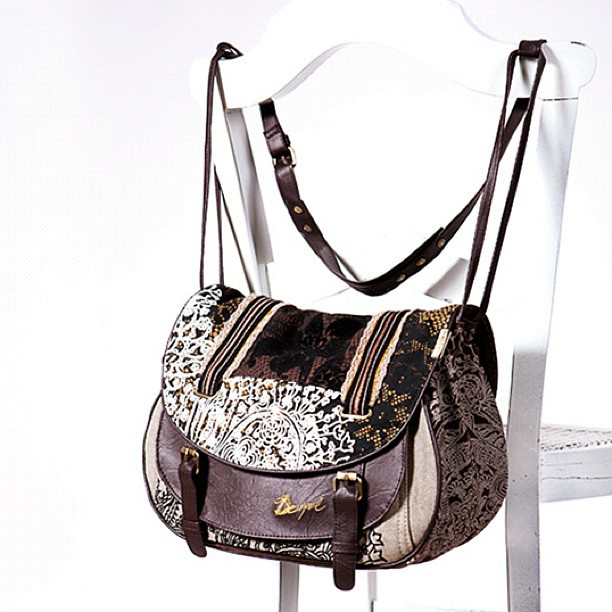
\includegraphics[width=0.9in, height=0.9in]{img/spam2} \label{fig:ob_inflamatory_histology}}
\subfloat{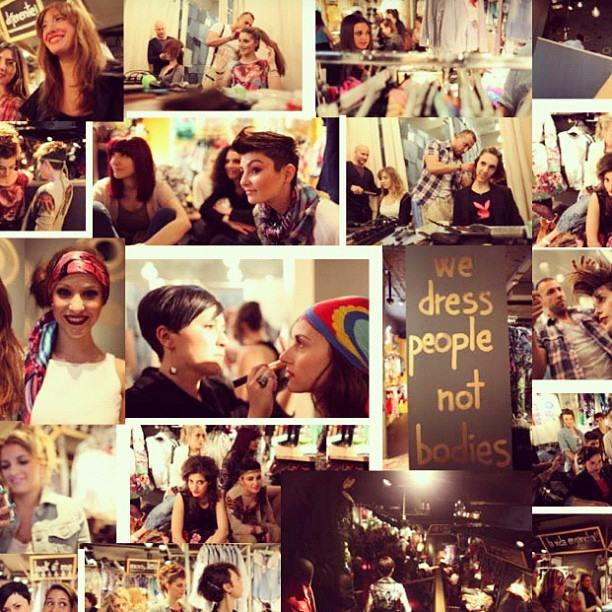
\includegraphics[width=0.9in, height=0.9in]{img/spam3} \label{fig:ob_inflamatory_histology}}\\
\subfloat{
\includegraphics[width=0.9in, height=0.9in]{img/spam4} \label{fig:ob_inflamatory_histology}}
\subfloat{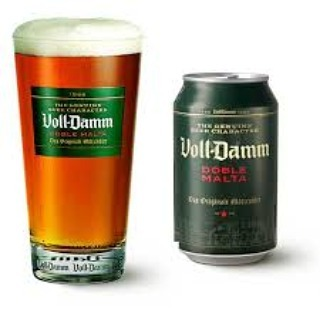
\includegraphics[width=0.9in, height=0.9in]{img/spam5} \label{fig:ob_inflamatory_histology}}
\subfloat{
\includegraphics[width=0.9in, height=0.9in]{img/spam6} \label{fig:ob_inflamatory_histology}}\\
\subfloat{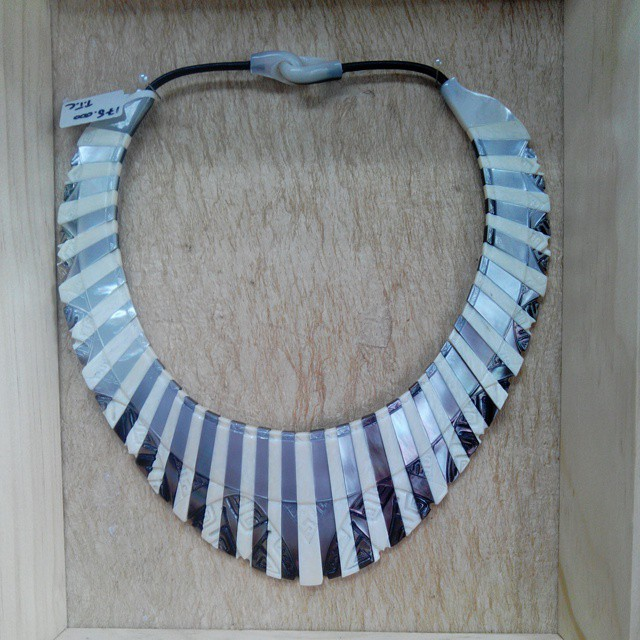
\includegraphics[width=0.9in, height=0.9in]{img/spam7} \label{fig:ob_inflamatory_histology}}
\subfloat{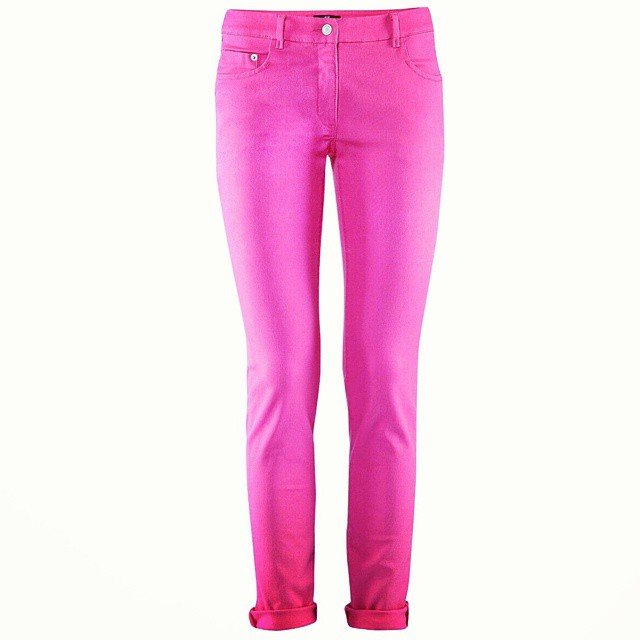
\includegraphics[width=0.9in, height=0.9in]{img/spam8} \label{fig:ob_inflamatory_histology}}
\subfloat{
\includegraphics[width=0.9in, height=0.9in]{img/spam9} \label{fig:ob_inflamatory_histology}}
\caption{Example images posted by Instagram users and tagged with Desigual's promotional hashtags (e.g. \#lavidaeschula)}
\label{fig:spamexamples}
\end{figure}

However, discovering valuable images on social media streams is challenging. The amount of images to process is huge and, while they help, user defined tags are scarce and noisy. The most part of current solutions rely on costly manual curation tasks over random samples. This way many contents are not even processed, and many valuable photos go unnoticed. 

This situation is aggravated by the huge amount of \textit{spam images}. In the context of UGC, we consider spam any image that, in the most usage scenarios, has no value neither as a knowledge carrier nor as a exploitable content. This includes images posted with commercial purposes, but also inappropriate images or very common images with low value such as photos of pets (Figure \ref{fig:spamexamples} shows some examples). Of course, this may be relative in some cases (e.g. for a pet food company).  

We propose using deep convolutional neural networks (CNNs) to automatically detect the most common types of spam images, facilitating their early filtering. We do not merge the different spam categories in order to enable a fine-grained filtering, as, as mentioned before, the definition of spam is relative to the usage scenario. 

TODO (LEONEL): A comment of the type of CNN, size of datasets.

We train the CNNs in a distributed manner, with the help of the Apache Spark cluster-computing framework, over MareNostrum, a petascale supercomputer. This implies several challenges, not only in terms of deployment but specially regarding scalability and proper configuration. Simply running on hundreds of cores may yield poor benefits or even degraded performance due to overheads. We deal with this issues and we have identifed solutions to potential inefficiencies of such a data-centric workload running over a compute-centric infrastructure.

TODO (RUBEN): SUMMARY OF CONTRIBUTIONS


\section{Related Work}
\label{sec:1}
The work presented in this paper is related to recent works attempting to facilitate the classification and search of images in social networks such as Instagram and Twitter. Some works, such as \cite{DBLP:journals/corr/ParkLK16}, \cite{conf/bigmm/TousTA15} or \cite{Denton:2015:UCH:2783258.2788576}, also apply image recognition techniques to enrich the metadata originally present in the images in order to facilitate their processing. All latest works rely on CNNs as an underlying technique. In our case, the applied image recognition techniques, while also relying in CNNs, are tuned for spam detection. TODO: Explain particularities of the approach (distributed, spark, etc.)
 
TODO (?): Something about the distributed part, including this ref: \cite{conf/bigdataconf/TousGTTGALBCV15}

\section{Spam recognition CNN architecture}

TODO (LEONEL): Layers, etc.

\section{Dataset}

TODO (?)

\section{Distributed training setup}

We trained the models in a distribued manner on MareNostrum, the Spanish Tier-0 supercomputer. It is an IBM System X iDataplex based on Intel Sandy Bridge EP processors at 2.6 GHz (two 8-core Intel Xeon processors E5-2670 per machine), 2 GB/core (32 GB/node). Currently the supercomputer consists of 48,896 Intel Sandy Bridge cores in 3,056 JS21 nodes, and 84 Xeon Phi 5110P in 42 nodes (not used in this work), with more than 104.6 TB of main memory and 2 PB of GPFS (General Parallel File System) disk storage. All compute nodes are interconnected through an Infiniband FDR10 network, with a non-blocking fat tree network topology. MareNostrum has a peak performance of 1.1 Petaflops.

While CNNs are trained more efficiently over GPUs, the availability of such huge computation power made us design a strategy for training our models over an HPC setup. The key element was Apache Spark \cite{zaharia2012}, a distributed computing framework that is already available at MareNostrum and provides a very convenient abstraction layer. Spark is an implementation of the so-called Resilient Distributed Dataset (RDD) abstraction, which hides the details of distribution and fault-tolerance for large collections of items. Spark is designed to avoid the file system as much as possible, retaining most data resident in distributed memory across phases in the same job. Such memory-resident feature stands to benefit many applications, such as machine learning or clustering, that require extensive reuse of results across multiple iterations. Memory usage is the key aspect of Spark and the main reason that it outperforms Hadoop for many applications. In order to be able to efficiently run a Spark cluster on the MareNostrum supercomputer (which runs an IBM LSF Platform workload manager), we employ the Spark4MN framework described in \cite{conf/bigdataconf/TousGTTGALBCV15}. 

As we were distributing computation over Spark, based on Java, we chose the DL4J framework TODO CITATION to be able to train our models in a distributed manner over this setup. DL4J is... TODO BREVE COMENTARIO


%At  June 2013, MareNostrum was positioned at  the 29th place in the TOP500 list of fastest supercomputers in the world.


%
\section{Results}
%
We have submitted and tested several hundreds of jobs to MareNostrum, but we describe only the results that are of significance. Our runs include an extensive  set of configurations; for brevity, when those parameters were shown to be either irrelevant or to have negligible effect, we use default values. Each experimental configuration was repeated at least 5 times. Unless otherwise stated, we report median values in seconds. 

TODO (Leonel)...

\subsection{Classification accuracy}
%

\begin{table}
\begin{center}\footnotesize 
\begin{tabular}{|c|c|c|c|c|c|}
\hline
tag & \#positives & \#total images & BoW & CNN & CNN-TL \\\hline\hline 
selfie & 295 & 9,254 &  72\% &  87\% &  93\%     \\\hline
group\_selfie & 98 & 8,982 &  76\% &  88\% &  95\%     \\\hline
spam & 319 & 9,298 &  69\% &  78\% &  91\%     \\\hline
burguer & 474 & 9,319 & 81\% &  89\% &  95\%     \\\hline
nails & 434 & 9,300 & 83\% &  92\% &  97\%     \\\hline
sushi & 571 & 9,491 & 86\% &  93\% &  96\%     \\\hline
\end{tabular} 
\end{center}
\caption{\footnotesize Training setup and results of some of the 100 new models that we have trained for image semantics recognition.}
\label{tags_accuracy}
\end{table}

\begin{figure}
\centering
\subfloat{
\includegraphics[width=0.9in, height=0.9in]{img/spam1} \label{fig:ob_inflamatory_histology}}
\subfloat{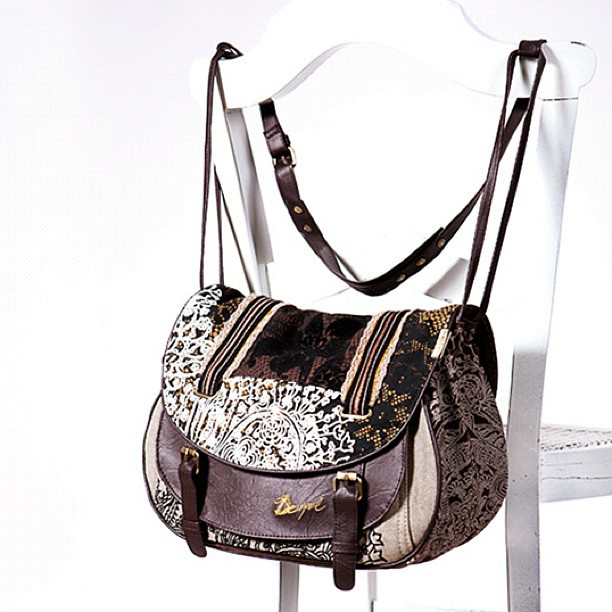
\includegraphics[width=0.9in, height=0.9in]{img/spam2} \label{fig:ob_inflamatory_histology}}
\subfloat{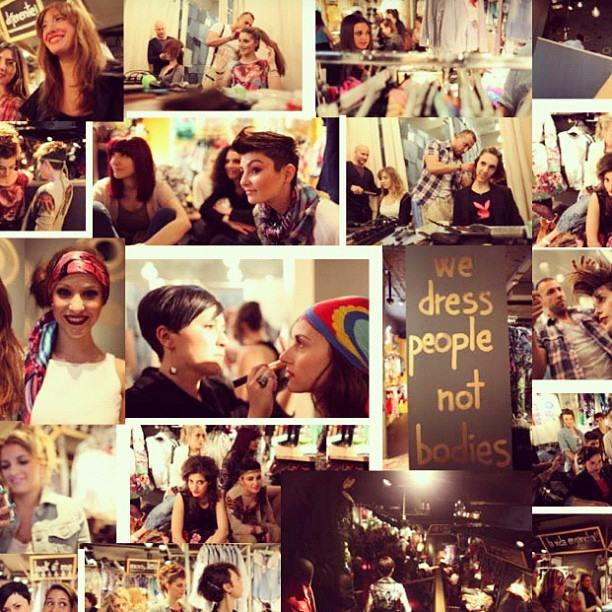
\includegraphics[width=0.9in, height=0.9in]{img/spam3} \label{fig:ob_inflamatory_histology}}\\
\subfloat{
\includegraphics[width=0.9in, height=0.9in]{img/spam4} \label{fig:ob_inflamatory_histology}}
\subfloat{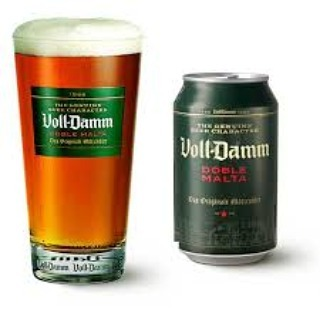
\includegraphics[width=0.9in, height=0.9in]{img/spam5} \label{fig:ob_inflamatory_histology}}
\subfloat{
\includegraphics[width=0.9in, height=0.9in]{img/spam6} \label{fig:ob_inflamatory_histology}}\\
\subfloat{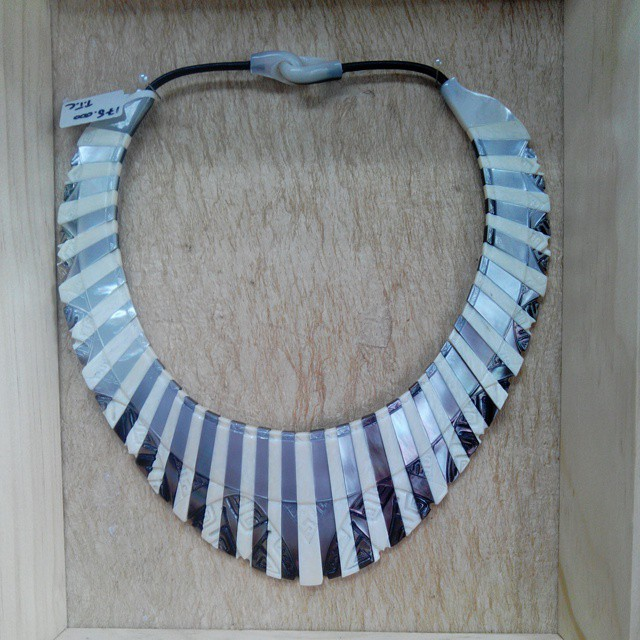
\includegraphics[width=0.9in, height=0.9in]{img/spam7} \label{fig:ob_inflamatory_histology}}
\subfloat{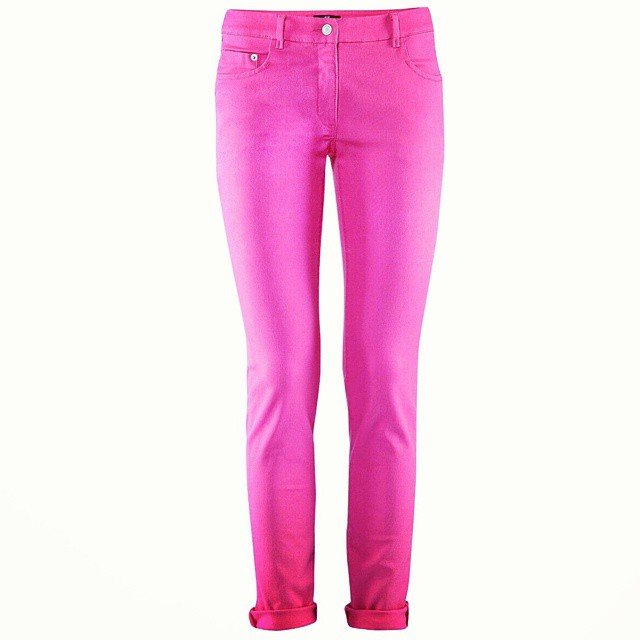
\includegraphics[width=0.9in, height=0.9in]{img/spam8} \label{fig:ob_inflamatory_histology}}
\subfloat{
\includegraphics[width=0.9in, height=0.9in]{img/spam9} \label{fig:ob_inflamatory_histology}}
\caption{Example true positives)}
\label{fig:spamexamples}
\end{figure}

\begin{figure}
\centering
\subfloat{
\includegraphics[width=0.9in, height=0.9in]{img/spam1} \label{fig:ob_inflamatory_histology}}
\subfloat{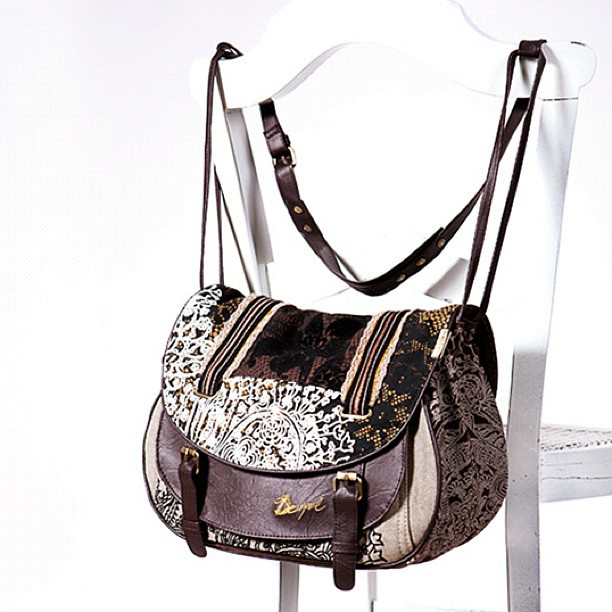
\includegraphics[width=0.9in, height=0.9in]{img/spam2} \label{fig:ob_inflamatory_histology}}
\subfloat{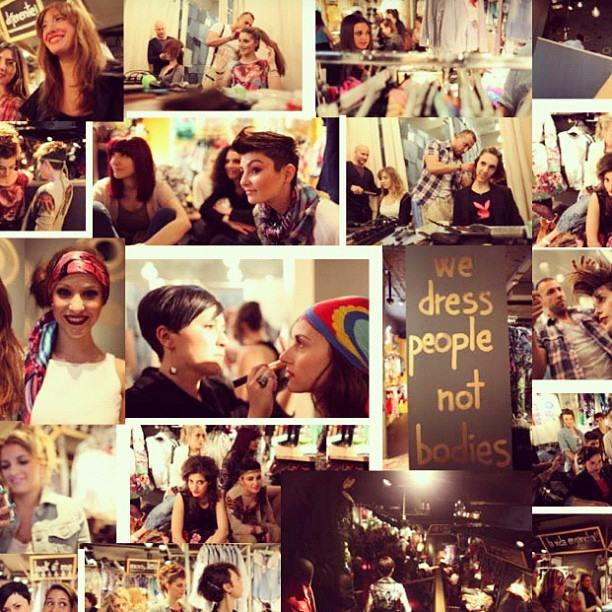
\includegraphics[width=0.9in, height=0.9in]{img/spam3} \label{fig:ob_inflamatory_histology}}\\
\subfloat{
\includegraphics[width=0.9in, height=0.9in]{img/spam4} \label{fig:ob_inflamatory_histology}}
\subfloat{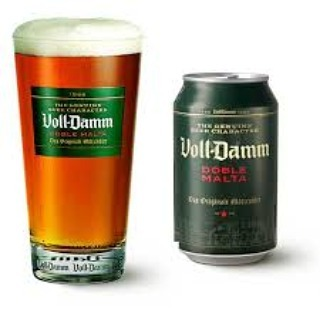
\includegraphics[width=0.9in, height=0.9in]{img/spam5} \label{fig:ob_inflamatory_histology}}
\subfloat{
\includegraphics[width=0.9in, height=0.9in]{img/spam6} \label{fig:ob_inflamatory_histology}}\\
\subfloat{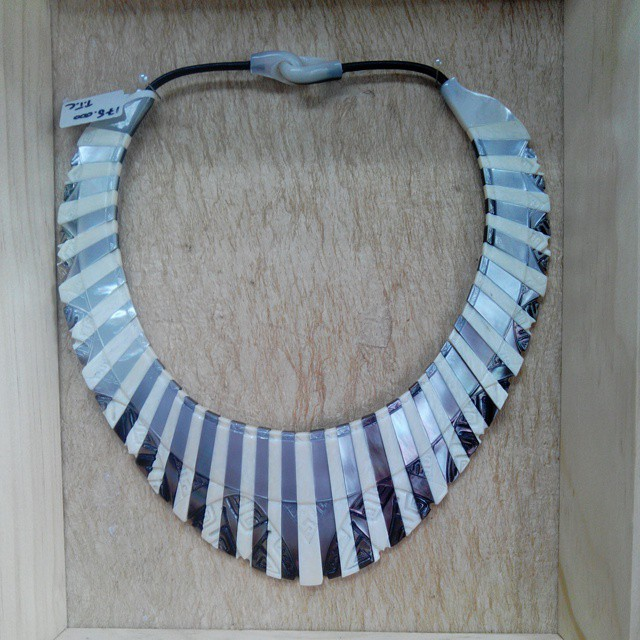
\includegraphics[width=0.9in, height=0.9in]{img/spam7} \label{fig:ob_inflamatory_histology}}
\subfloat{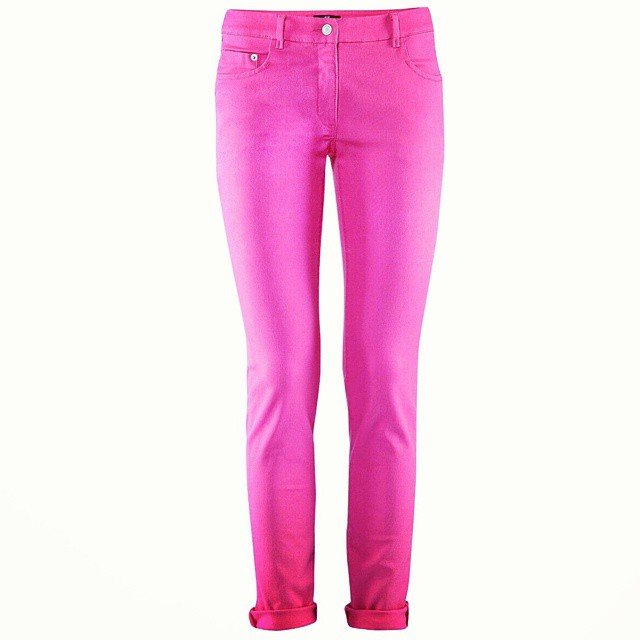
\includegraphics[width=0.9in, height=0.9in]{img/spam8} \label{fig:ob_inflamatory_histology}}
\subfloat{
\includegraphics[width=0.9in, height=0.9in]{img/spam9} \label{fig:ob_inflamatory_histology}}
\caption{Example false positives)}
\label{fig:spamexamples}
\end{figure}

\begin{figure}
\centering
\subfloat{
\includegraphics[width=0.9in, height=0.9in]{img/spam1} \label{fig:ob_inflamatory_histology}}
\subfloat{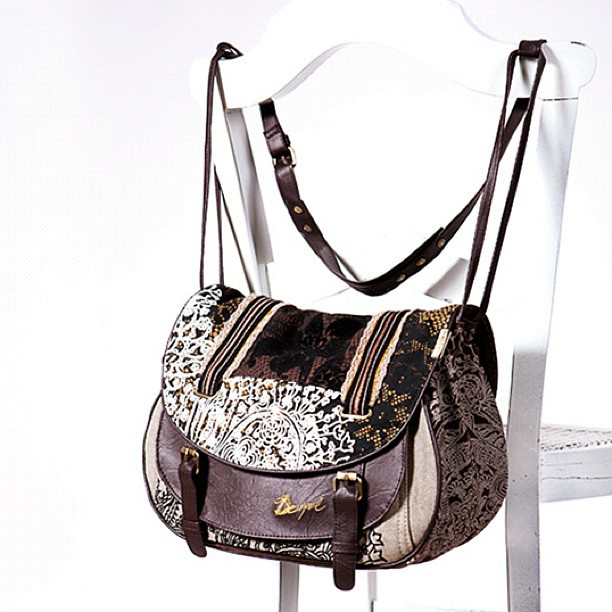
\includegraphics[width=0.9in, height=0.9in]{img/spam2} \label{fig:ob_inflamatory_histology}}
\subfloat{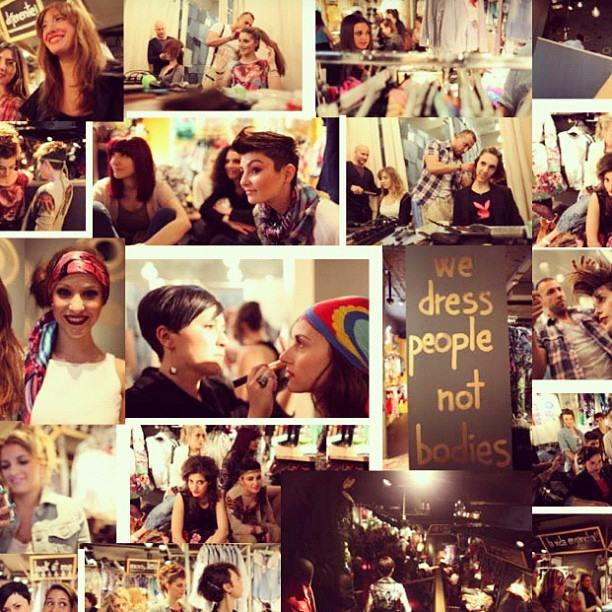
\includegraphics[width=0.9in, height=0.9in]{img/spam3} \label{fig:ob_inflamatory_histology}}\\
\subfloat{
\includegraphics[width=0.9in, height=0.9in]{img/spam4} \label{fig:ob_inflamatory_histology}}
\subfloat{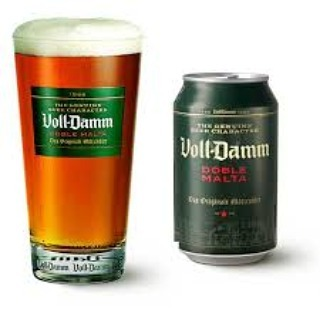
\includegraphics[width=0.9in, height=0.9in]{img/spam5} \label{fig:ob_inflamatory_histology}}
\subfloat{
\includegraphics[width=0.9in, height=0.9in]{img/spam6} \label{fig:ob_inflamatory_histology}}\\
\subfloat{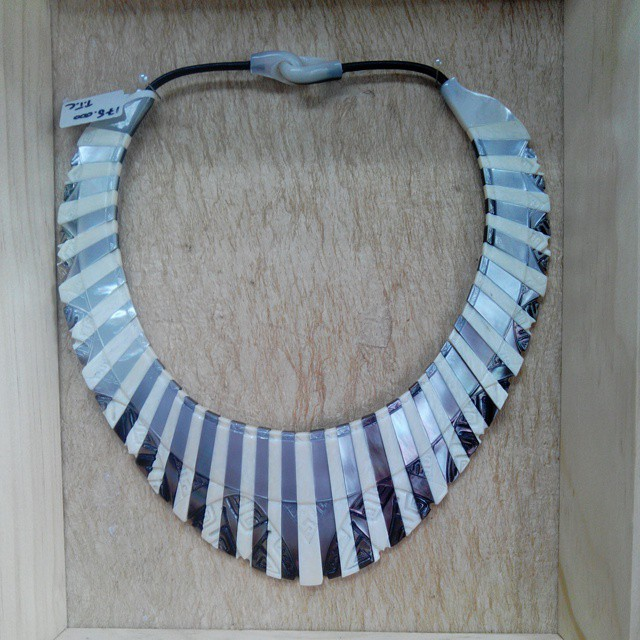
\includegraphics[width=0.9in, height=0.9in]{img/spam7} \label{fig:ob_inflamatory_histology}}
\subfloat{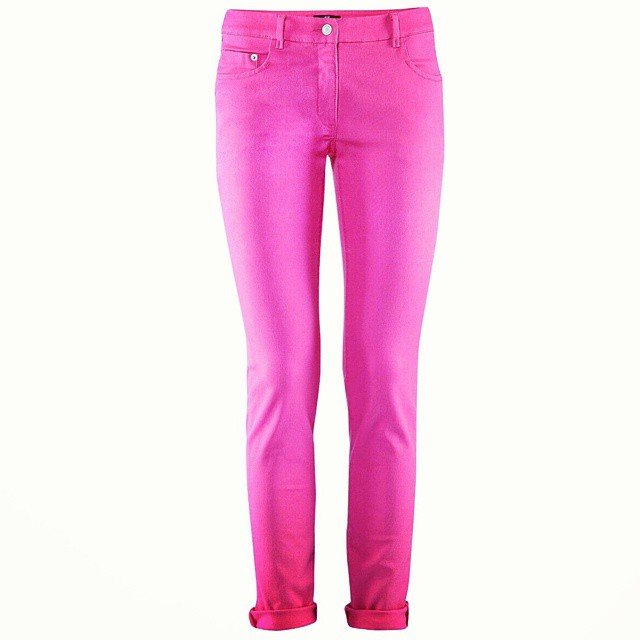
\includegraphics[width=0.9in, height=0.9in]{img/spam8} \label{fig:ob_inflamatory_histology}}
\subfloat{
\includegraphics[width=0.9in, height=0.9in]{img/spam9} \label{fig:ob_inflamatory_histology}}
\caption{Example false negatives)}
\label{fig:spamexamples}
\end{figure}

\subsection{Performance and Scalability}
The main goal of these experiments is to evaluate the speed-up, scale-up, and size-up properties of the proposed distributed training strategy. To this end, we use datasets up to hundreds of GBs TODO of raw data. The size of RDDs is reported to be 2-5 times larger than that; in our experiments 400GBs of data in the sort-by-key application correspond to an RDD of 1TB.
 The cluster sizes range from 8 cores up to 1024 (i.e., 64 machines)...TODO

\subsubsection{speed-up} In the first set of experiments, we keep the input dataset constant and we increase the size of nodes/cores running the Spark application; whenever we refer to nodes, we mean  MareNostrum machines that run the executors, while the driver always runs on a separate machine; each machine is equipped with 16 cores and 32 GB of RAM. The results from 128 (8 nodes) up to 512 cores (32 nodes) are shown in Figure \ref{fig:speedup1}, where we can see that for large datasets in terms of number of records, the training can scale well. In the figure, we present the performance for the most efficient configurations; we discuss these configurations in detail later. TODO

\begin{figure}[tb!]
\begin{center}
\centerline{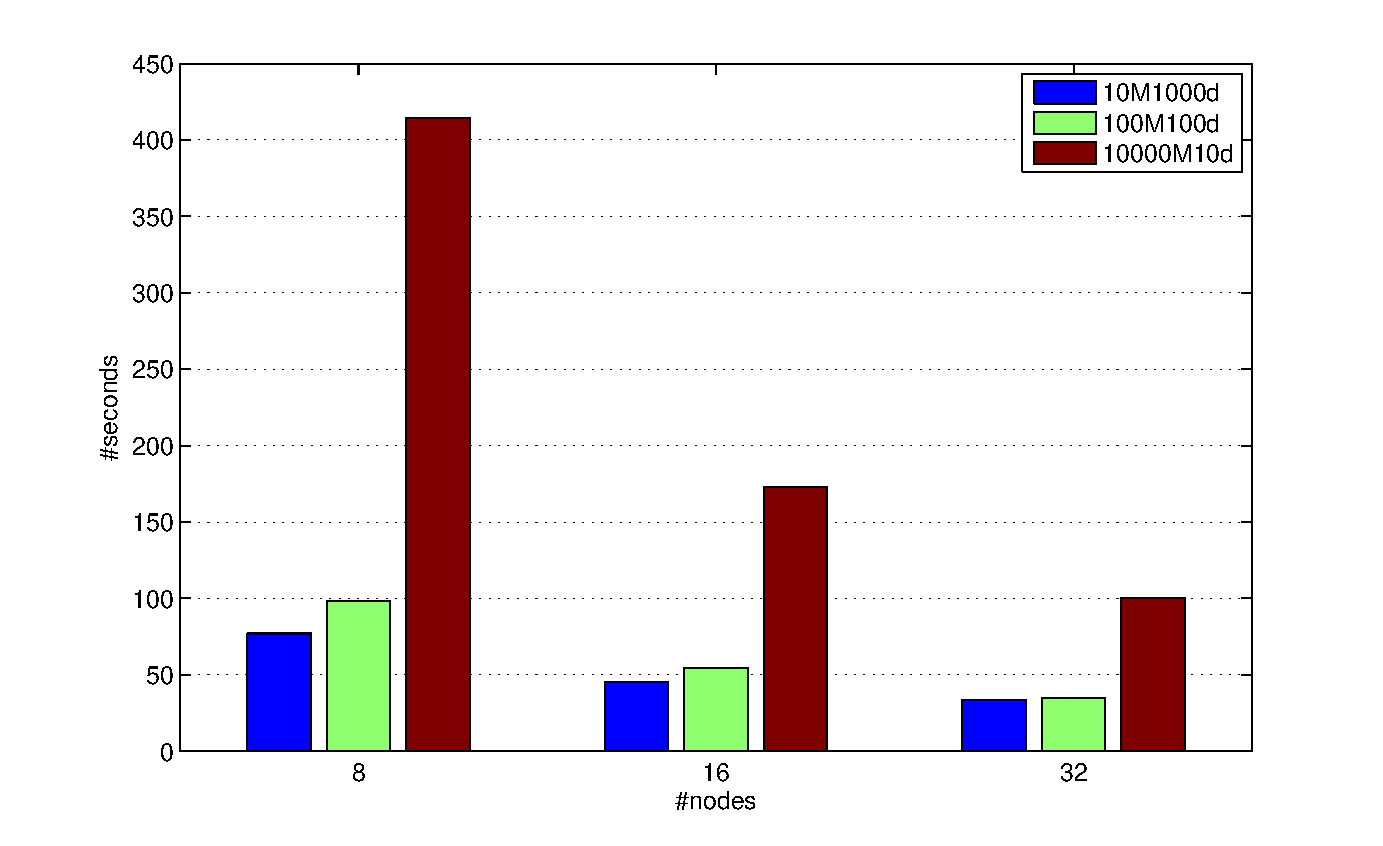
\includegraphics[width=0.75\linewidth]{img/speedup1.pdf}}
\caption{Times for training....}
\label{fig:speedup1}
\end{center}
\vspace{-0.5cm}
\end{figure}

\subsubsection{scale-up} We process the same datasets, and we now modify both the number of records and the number of machines, i.e., the infrastructure scales-out. .... The results are shown in Figure \ref{fig:scaleup1}(top). In this figure, we show both the average and the median values. Ideally, all the plots should be horizontal; our system behaves closely to that. ....

\begin{figure}[tb!]
\begin{center}
\centerline{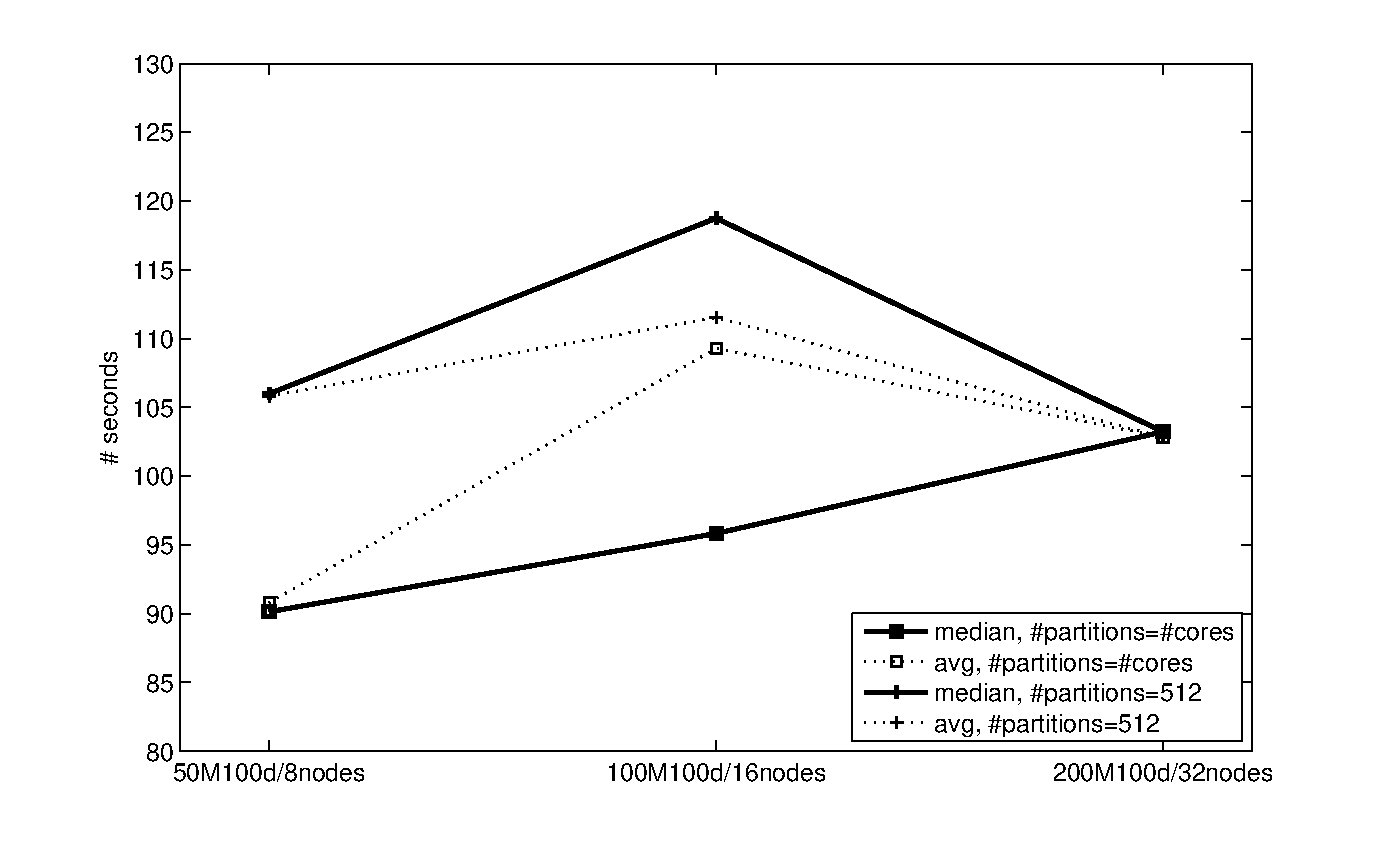
\includegraphics[width=0.75\linewidth]{img/scaleup1.pdf}}
\caption{Times for training....}
\label{fig:speedup1}
\end{center}
\vspace{-0.5cm}
\end{figure}

\subsubsection{size-up} We perform a third set of experiments, to assess the capability of sizing-up. We keep the number of nodes constant (either 16 or 32), and we gradually increase the dataset from 100GBs to 200GBs (raw data sizes). As shown in Figure \ref{fig:sizeup1}(bottom), Spark4MN exhibits a behavior where the curves are (almost) linear. ....

\begin{figure}[tb!]
\begin{center}
\centerline{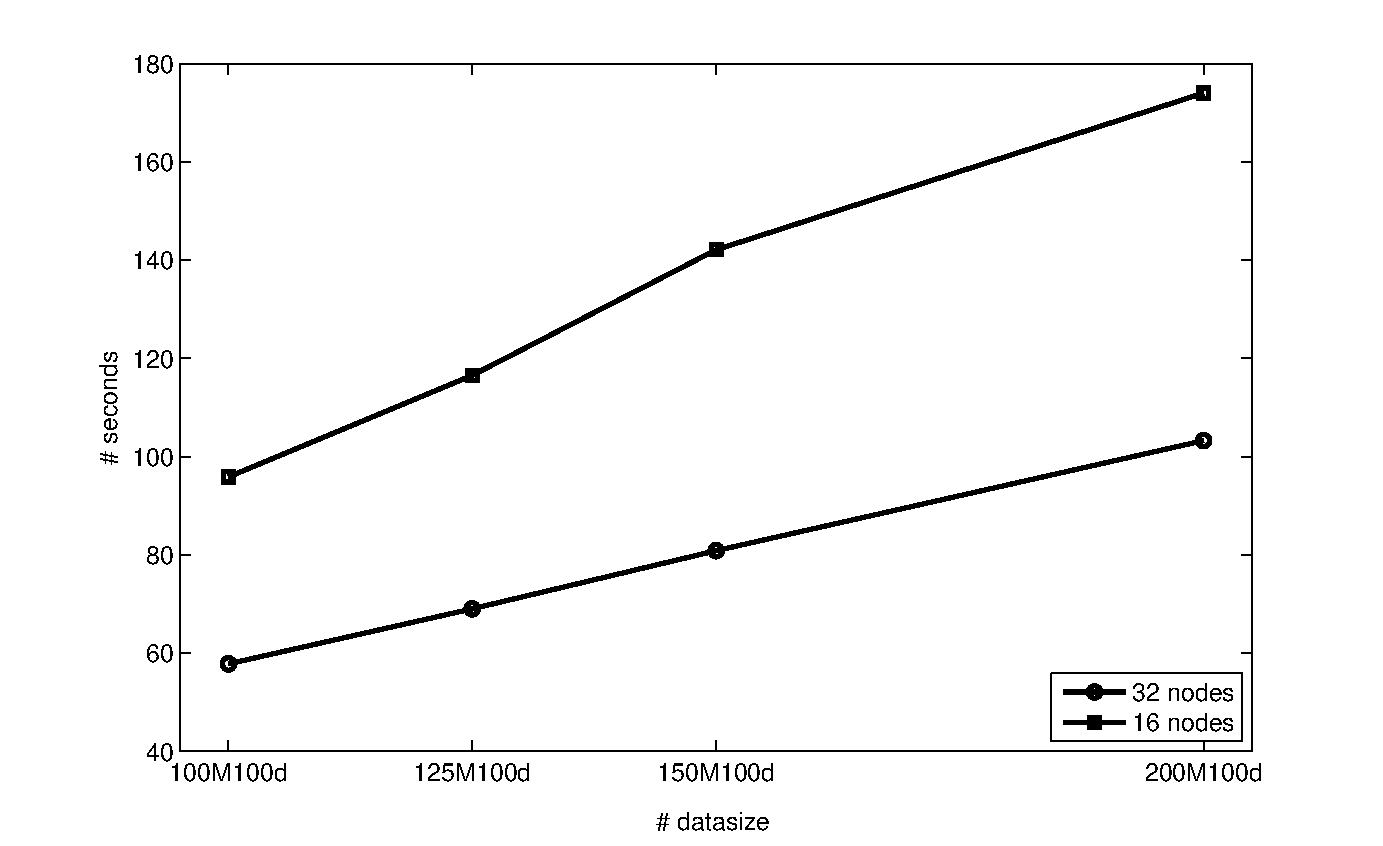
\includegraphics[width=0.75\linewidth]{img/sizeup1.pdf}}
\caption{Times for training....}
\label{fig:speedup1}
\end{center}
\vspace{-0.5cm}
\end{figure}

%
\section{Conclusions}
%
The research work presented in this paper analyzes the usage of distributed deep convolutional neural networks (CNNs) for ..... 

TODO (?)

\begin{acknowledgements}
This work is partially supported by the Spanish Ministry of Economy and Competitivity under contract TIN2015-65316-P and by the SGR programme (2014-SGR-1051) of the Catalan Government.
\end{acknowledgements}

\bibliographystyle{spmpsci}
\bibliography{refs}

\end{document}

